\documentclass{scrartcl}
\usepackage[a4paper, total={6in, 10in}]{geometry}
\usepackage[ngerman]{babel}

\usepackage{xcolor}
\usepackage{graphicx}
\usepackage{multirow} % Wichtig: Fügen Sie dieses Paket in Ihrer Präambel hinzu!
\usepackage{array} % Oft nützlich in Verbindung mit tabularx

\usepackage{amsmath}
\usepackage{amsthm}
\usepackage{amssymb}
\usepackage{algorithm}
\usepackage{algpseudocode}

\newtheorem{satz}{Satz}[section]
\newtheorem{lemma}{Lemma}[section]

\makeatletter
\renewcommand{\ALG@name}{Algorithmus}
\makeatother
\algrenewcommand\algorithmicrequire{\textbf{Eingabe:}}
\algrenewcommand\algorithmicensure{\textbf{Ausgabe:}}

\title{Matrixmultiplikation von \normalfont\scshape{Strassen}}
\author{Stephan Epp\\\texttt{hjstephan86@gmail.com}}
\date{\today}

\begin{document}
\maketitle
\begin{abstract}
	Diese Arbeit untersucht den \textsc{Strassen}-Algorithmus zur Matrixmultiplikation, der eine schnellere Laufzeit von $O(n^{\log_2 7})$ gegenüber dem Standardalgorithmus mit $O(n^3)$ hat. Die Rekurrenzgleichung des Algorithmus wird dazu hergeleitet und gelöst. Der Algorithmus wird in Pseudocode präsentiert und seine Korrektheit exemplarisch demonstriert. Experimentelle Ergebnisse einer Python-Implementierung zeigen, dass \textsc{Strassen} für kleine Matrizen aufgrund des Rekursionsaufwands zunächst langsamer ist, für größere Matrizen (ab $n=256$) die Standardmethode jedoch übertrifft. \textsc{Strassen}'s Algorithmus wird erweitert zu \textsc{Strassen-25}, um die Anzahl der Matrixmultiplikationen von sieben auf fünf zu reduzieren. Es wird gezeigt, dass es keinen Teile-und-Herrsche Algorithmus geben kann, der weniger als fünf Matrixmultiplikationen benötigt. Zudem wird das \textit{optimale Teile-und-Herrsche Prinzip} betrachtet und gezeigt, dass es die effizienteste Methode ist, um geeignete Probleme zu lösen. Es wird gezeigt, dass zwei $n \times n$ Matrizen nicht schneller multipliziert werden können als in $O(n^{2.3219})$. Es wird gezeigt, dass das optimale Teile-und-Herrsche Prinzip optimal ist.
\end{abstract}

\section{Laufzeit}
Beim Algorithmus von \textsc{Strassen} für die Multiplikation von zwei $n \times n$ Matrizen lautet die Rekurrenzgleichung zur Ermittlung der Laufzeit $T(n)$ des Algorithmus
\begin{align*}
	T(n) = 7 \: T(\tfrac{n}{2}) + c\: n^2.
\end{align*}
Der Algorithmus halbiert in jedem rekursiven Aufruf die beiden $n \times n$ Matrizen zu vier $\tfrac{n}{2} \times \tfrac{n}{2}$ Matrizen. Substituieren wir $n$ durch $\tfrac{n}{2}$, erhalten wir für
\begin{align*}
	T(\tfrac{n}{2}) &= 7 \: T(\tfrac{n}{4}) + c(\tfrac{n}{2})^2 = 7 \: T(\tfrac{n}{4}) + \tfrac{c}{4}n^2.
\end{align*}
Nach dem \textit{ersten} rekursiven Aufruf erhalten wir mit $T(\frac{n}{2})$ eingesetzt in $T(n)$ dann
\begin{align*}
	T(n) &= 7 \: (7 \: T(\tfrac{n}{4}) + \tfrac{c}{4} \: n^2) + c n^2 \\
	&= 7^2\: T(\tfrac{n}{4}) + \tfrac{7}{4} \: cn^2 + c n^2.
\end{align*}
Mit dem \textit{zweiten} rekursiven Aufruf werden die vier $\tfrac{n}{2} \times \tfrac{n}{2}$ Matrizen wieder halbiert zu acht $\tfrac{n}{4} \times \tfrac{n}{4}$ Matrizen. Damit ist
\begin{align*}
	T(\tfrac{n}{4}) &= 7 \: T(\tfrac{n}{8}) + c(\tfrac{n}{4})^2 = 7 \: T(\tfrac{n}{8}) + \tfrac{c}{16}n^2.
\end{align*}
Wird $T(\tfrac{n}{4})$ eingesetzt in $T(n)$ ergibt sich
\begin{align*}
	T(n) &= 7^2\: (7 \: T(\tfrac{n}{8}) + \tfrac{c}{16}n^2) + \tfrac{7}{4}cn^2 + c n^2 \\
	&= 7^3\: T(\tfrac{n}{2^3}) + \tfrac{7^2}{4^2}cn^2 + \tfrac{7}{4}cn^2 + c n^2.
\end{align*}
Betrachten wir nun den $k$-ten rekursiven Aufruf finden wir für 
\begin{align*}
	T(n) = 7^k \: T \: \big(\tfrac{n}{2^k}\big) + cn^2 \: \sum_{i = 0}^{k-1} \bigg(\frac{7}{4}\bigg)^i.
\end{align*}
Zur Vereinfachung belassen wir es bei dem $k$-ten rekursiven Aufruf auch in $T(n)$ bei $k$ und nicht $k + 1$. Kleinere Matrizen als $1 \times 1$ Matrizen gibt es nicht, daher können die $n \times n$ Matrizen nur $k$ mal halbiert werden. Der größte Wert, den $k$ annehmen kann, ist $k = \log_{2}n$. Damit ist
\begin{align*}
	\vphantom{\rule{0pt}{2.5ex}} T(n) &= 7^{\log_{2}n} \: T\Big(\frac{n}{2^{\log_{2}n}}\Big) + cn^2 \: \sum_{i = 0}^{\log_{2}n-1} \left(\tfrac{7}{4}\right)^i \\
	\vphantom{\rule{0pt}{2.5ex}} &= n^{\log_{2}7} \: T(1) + cn^2 \:\frac{\left(\tfrac{7}{4}\right)^{\log_{2}n} - 1}{\tfrac{7}{4} - 1} \\
	\vphantom{\rule{0pt}{2.5ex}} &= O\left(n^{2.8074}\right) + cn^2 \left(\tfrac{7}{4}\right)^{\log_{2}n} \\
	\vphantom{\rule{0pt}{2.5ex}} &= O\left(n^{2.8074}\right) + cn^2 \cdot n^{\log_{2}\tfrac{7}{4}} \\
	\vphantom{\rule{0pt}{2.5ex}} &= O\left(n^{2.8074}\right) + cn^{2.8074} \\
	\vphantom{\rule{0pt}{2.5ex}} &= O\left(n^{2.8074}\right).
\end{align*}

\section{Algorithmus}
Es folgt der Algorithmus \ref{alg:strassen} von \textsc{Strassen}  als Pseudocode. Als Eingabe erhalten wir zwei $n \times n$ Matrizen. Der Einfachheit halber wird angenommen, dass $n$ eine Zweierpotenz ist.
\begin{algorithm}
	\caption{\textsc{Strassen}$(A, B)$}
	\label{alg:strassen}
	\begin{algorithmic}[1]
		\Require $\langle A, B \rangle$, mit $n \times n$ Matrizen $A$, $B$, $n = 2^k$, $k \in \mathbb{N}$
		\Ensure $\langle C \rangle$, mit Produktmatrix $C = AB$
		\If{$n = 1$} $C = AB$ %\Comment{Skalarmultiplikation}
		\State \textbf{return} $C$
		\EndIf
		%\Comment{Matrizen in $n/2 \times n/2$ Blöcke unterteilen}
		\State $A = \begin{pmatrix} A_{11} & A_{12} \\ A_{21} & A_{22} \end{pmatrix}$
		\State $B = \begin{pmatrix} B_{11} & B_{12} \\ B_{21} & B_{22} \end{pmatrix}$
		%\Comment{Berechne die 7 Produkte rekursiv}
		\State $P_1 = \textsc{Strassen}(A_{11} + A_{22}, B_{11} + B_{22})$
		\State $P_2 = \textsc{Strassen}(A_{21} + A_{22}, B_{11})$
		\State $P_3 = \textsc{Strassen}(A_{11}, B_{12} - B_{22})$
		\State $P_4 = \textsc{Strassen}(A_{22}, B_{21} - B_{11})$
		\State $P_5 = \textsc{Strassen}(A_{11} + A_{12}, B_{22})$
		\State $P_6 = \textsc{Strassen}(A_{21} - A_{11}, B_{11} + B_{12})$
		\State $P_7 = \textsc{Strassen}(A_{12} - A_{22}, B_{21} + B_{22})$
		% \Comment{Berechne die Blöcke von $C$}
		\State $C_{11} = P_1 + P_4 - P_5 + P_7$
		\State $C_{12} = P_3 + P_5$
		\State $C_{21} = P_2 + P_4$
		\State $C_{22} = P_1 - P_2 + P_3 + P_6$
		\State \textbf{return} $C = \begin{pmatrix} C_{11} & C_{12} \\ C_{21} & C_{22} \end{pmatrix}$
	\end{algorithmic}
\end{algorithm}
Zu Beginn prüfen wir, ob die Größe der Matrizen bereits den Wert $1$ hat. Haben die Matrizen den Wert $1$, geben wir das Produkt $A B$ zurück. In Zeile 4 und 5 werden die Matrizen $A$ und $B$ so definiert, dass in den Zeilen 6 bis 12 die 7 Matrixmultiplikationen jeweils durchgeführt werden. In den Zeilen 13 bis 16 werden 4 Matrizen $C_{ij}$ durch Addition und Subtraktion der Matrizen $A_{ij}$ berechnet und in Zeile 17 Matrix $C$ als Ergebnis zurückgegeben.

Als Idee zum Beweis der Korrektheit betrachten wir das Produkt $A \cdot B$ der zwei Matrizen $A$ und $B$ mit
\begin{align*}
	A = \begin{pmatrix} a & b \\ c & d \end{pmatrix} \quad \text{und} \quad B = \begin{pmatrix} e & f \\ g & h \end{pmatrix}.
\end{align*}
Zur Vereinfachung beinhalten die Matrizen nur skalare Werte. Das Ergebnis $C = A \cdot B$ ist
\begin{align*}
	C = \begin{pmatrix} ae + bg & af + bh \\ ce + dg & cf + dh \end{pmatrix}.
\end{align*}
Der Algorithmus von \textsc{Strassen} berechnet $P_r$ mit
\[
\begin{array}{ll}
	P_1 = \textsc{Strassen}(a + d, e + h) & = ae + ah + de + dh, \\
	P_2 = \textsc{Strassen}(c + d, e)     & = ce + de, \\
	P_3 = \textsc{Strassen}(a, f - h)     & = af - ah, \\
	P_4 = \textsc{Strassen}(d, g - e)     & = dg - de, \\
	P_5 = \textsc{Strassen}(a + b, h)     & = ah + bh, \\
	P_6 = \textsc{Strassen}(c - a, e + f) & = ce + cf - ae - af, \\
	P_7 = \textsc{Strassen}(b - d, g + h) & = bg + bh - dg - dh.
\end{array}
\]
Dann werden $C_{ij}$ berechnet mit
\[
\begin{array}{ll}
	C_{11} = P_1 + P_4 - P_5 + P_7 & = ae + bg, \\
	C_{12} = P_3 + P_5 & = af + bh, \\
	C_{21} = P_2 + P_4 & = ce + dg, \\
	C_{22} = P_1 - P_2 + P_3 + P_6 & = cf + dh,
\end{array}
\]
wobei z.B. $ C_{11} = (ae + ah + de + dh) + (dg - de) - (ah + bh) + (bg + bh - dg - dh) = ae + bg$. Für einen formalen Beweis der Korrektheit verzichten wir auf die vollständige Induktion über $n \in \mathbb{N}$ der $n \times n$ Matrizen.

\section{Experimentelle Ergebnisse}
Um die theoretische Laufzeitanalyse von \textsc{Strassen}s Algorithmus zu überprüfen, wurde eine Python-Implementierung des Algorithmus erstellt und deren Performance mit der einer Standard-Matrixmultiplikation verglichen. Die Experimente wurden für Matrizen unterschiedlicher Größe ($n$) durchgeführt, wobei $n$ von 4 bis 256 in Schritten von 4 variiert wurde. Für jede Matrixgröße wurden 5 Messungen (Trials) durchgeführt und die durchschnittliche Laufzeit ermittelt.
\begin{table}[h!]
	\centering
	\caption{Vergleich der Matrixmultiplikationen}
	\label{tab:strassen-results}
	\begin{tabular}{c|m{3.3cm}|m{3.3cm}}
		\hline
		\multirow{2}{*}{$n$} & \multicolumn{2}{c}{Durchschnittliche Laufzeit (s)} \\ % Multicolumn für die Überschrift
		\cline{2-3} % Linie unter der Multicolumn
		& Standard & \textsc{Strassen} \\ % Unterüberschrift
		\hline
		\hline
		4 & 0.000027 & 0.000045 \\ 
		8 & 0.000101 & 0.000142 \\ 
		12 & 0.000312 & 0.000698 \\ 
		16 & 0.000708 & 0.000808 \\ 
		20 & 0.001350 & 0.004538 \\  
		24 & 0.002304 & 0.004827 \\ 
		28 & 0.003644 & 0.005236 \\ 
		32 & 0.005369 & 0.005674 \\ 
		36 & 0.007291 & 0.035827 \\ 
		40 & 0.010007 & 0.036722 \\ 
		44 & 0.013256 & 0.037815 \\ 
		48 & 0.017039 & 0.038888 \\ 
		52 & 0.021834 & 0.034057 \\ 
		\textcolor{orange}{56} & \textcolor{orange}{0.013749} & \textcolor{orange}{0.020460} \\ 
		60 & 0.016938 & 0.020990 \\ 
		64 & 0.020041 & 0.021484 \\ 
		\vdots & \vdots & \vdots \\ 
		% 68 & 0.024157 & 0.133145 \\ % Auskommentierte Datenzeile
		% 72 & 0.028486 & 0.133083 \\ % Auskommentierte Datenzeile
		% 76 & 0.033549 & 0.143920 \\ % Auskommentierte Datenzeile
		% 80 & 0.039826 & 0.141013 \\ % Auskommentierte Datenzeile
		% 84 & 0.045262 & 0.141792 \\ % Auskommentierte Datenzeile
		% 88 & 0.051738 & 0.152629 \\ % Auskommentierte Datenzeile
		% 92 & 0.059471 & 0.146050 \\ % Auskommentierte Datenzeile
		% 96 & 0.067689 & 0.147936 \\ % Auskommentierte Datenzeile
		% 100 & 0.076471 & 0.162647 \\ % Auskommentierte Datenzeile
		% 104 & 0.087148 & 0.154874 \\ % Auskommentierte Datenzeile
		% 108 & 0.095150 & 0.155554 \\ % Auskommentierte Datenzeile
		% 112 & 0.107501 & 0.158186 \\ % Auskommentierte Datenzeile
		% 116 & 0.118892 & 0.171497 \\ % Auskommentierte Datenzeile
		% 120 & 0.131730 & 0.165475 \\ % Auskommentierte Datenzeile
		% 124 & 0.148736 & 0.166968 \\ % Auskommentierte Datenzeile
		% 128 & 0.161912 & 0.179074 \\ % Auskommentierte Datenzeile
		% 132 & 0.175445 & 0.999888 \\ % Auskommentierte Datenzeile
		% 136 & 0.191708 & 1.045382 \\ % Auskommentierte Datenzeile
		% 140 & 0.217163 & 1.082742 \\ % Auskommentierte Datenzeile
		% 144 & 0.233093 & 1.084697 \\ % Auskommentierte Datenzeile
		% 148 & 0.256793 & 1.078266 \\ % Auskommentierte Datenzeile
		% 152 & 0.272154 & 1.076065 \\ % Auskommentierte Datenzeile
		% 156 & 0.310149 & 1.115063 \\ % Auskommentierte Datenzeile
		% 160 & 0.324504 & 1.094453 \\ % Auskommentierte Datenzeile
		% 164 & 0.343517 & 1.101307 \\ % Auskommentierte Datenzeile
		% 168 & 0.363632 & 1.107035 \\ % Auskommentierte Datenzeile
		% 172 & 0.391884 & 1.117648 \\ % Auskommentierte Datenzeile
		% 176 & 0.418512 & 1.160525 \\ % Auskommentierte Datenzeile
		% 180 & 0.448960 & 1.159266 \\ % Auskommentierte Datenzeile
		% 184 & 0.471133 & 1.147314 \\ % Auskommentierte Datenzeile
		% 188 & 0.513541 & 1.139447 \\ % Auskommentierte Datenzeile
		% 192 & 0.542235 & 1.151873 \\ % Auskommentierte Datenzeile
		% 196 & 0.571728 & 1.158231 \\ % Auskommentierte Datenzeile
		% 200 & 0.608602 & 1.184203 \\ % Auskommentierte Datenzeile
		% 204 & 0.661712 & 1.198355 \\ % Auskommentierte Datenzeile
		% 208 & 0.683460 & 1.221877 \\ % Auskommentierte Datenzeile
		% 212 & 0.751752 & 1.258453 \\ % Auskommentierte Datenzeile
		% 216 & 0.793948 & 1.281702 \\ % Auskommentierte Datenzeile
		% 220 & 0.810436 & 1.224457 \\ % Auskommentierte Datenzeile
		% 224 & 0.864762 & 1.219905 \\ % Auskommentierte Datenzeile
		% 228 & 0.909023 & 1.232622 \\ % Auskommentierte Datenzeile
		% 232 & 0.962290 & 1.250792 \\ % Auskommentierte Datenzeile
		% 236 & 1.000335 & 1.258274 \\ % Auskommentierte Datenzeile
		240 & 1.055068 & 1.256394 \\ 
		244 & 1.105579 & 1.272495 \\ 
		248 & 1.158183 & 1.285980 \\ 
		252 & 1.221187 & 1.295652 \\ 
		\textcolor{red}{256} & \textcolor{red}{1.298067} & \textcolor{red}{1.286444} \\
		\hline
	\end{tabular}
\end{table}
Ein interner Schwellwert (threshold) von 32 wurde für \textsc{Strassen}s Algorithmus festgelegt, was bedeutet, dass für Matrizen, deren Größe kleiner oder gleich 32 ist, auf die Standard-Matrixmultiplikation umgeschaltet wird, um den zusätzliche Aufwand der Rekursion zu reduzieren. Die Systemauslastung vor Beginn der Experimente betrug 0,0\% CPU-Auslastung bei 3.38 GB verwendetem RAM von insgesamt 7.01 GB. Nach Abschluss der Experimente betrug die CPU-Auslastung 3.8\% und der verwendete RAM 3.43 GB, was auf eine moderate Systemauslastung während der Messungen hinweist. Die Messergebnisse sind in Tabelle \ref{tab:strassen-results} zusammengefasst.

Aus der Tabelle lässt sich ablesen, dass für kleine Matrizen (z.B. $n \le 64$) die Standard-Matrixmultiplikation tendenziell schneller war oder eine vergleichbare Performance wie \textsc{Strassen}s Algorithmus aufwies. Dies ist auf den zusätzlichen Aufwand der Rekursion und der zusätzlichen Matrixadditionen/-subtraktionen bei \textsc{Strassen}s Algorithmus zurück-zuführen. Insbesondere ist der Sprung in der Laufzeit des Algorithmus bei $n=36$ (nach dem eingestellten Schwellenwert von $n=32$) auffällig, was den Wechsel von der optimierten Basis-Multiplikation zur rekursiven Struktur widerspiegelt. Erst ab $n=256$ übertrifft \textsc{Strassen} die Standardmultiplikation leicht. Die tatsächliche Laufzeit wird jedoch stark vom gewählten Schwellwert und der Effizienz der Implementierung der Basisfälle beeinflusst.

\begin{figure}[h]
	\centering
	\caption{Vergleich der Laufzeit der Matrixmultiplikationen}
	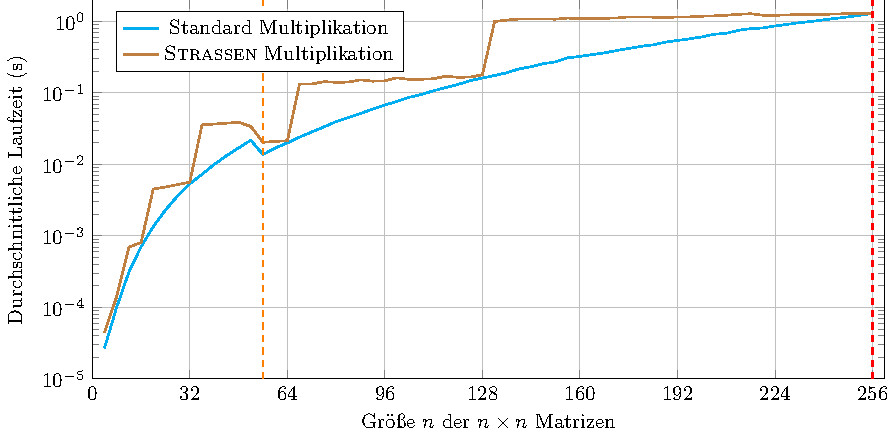
\includegraphics[width=1.0\textwidth]{results.pdf}
	\label{fig:time-comparison}
\end{figure}

Die Abbildung \ref{fig:time-comparison} zeigt die Verläufe der benötigten Rechenzeit beider Matrixmultiplikationen. Für $n = 56$ waren sowohl die Standard als auch \textsc{Strassen}s Multiplikation schneller als für vorherige $n < 56$. \textsc{Strassen} verwendet 7 Matrixmultiplikationen für zwei Matrizen der Größe $n \times n$. Lässt sich die Anzahl der benötigten Matrixmultiplikationen reduzieren?

\section{Optimierung}
Um die Anzahl der benötigten Matrixmultiplikationen von 7 auf 5 zu reduzieren, wird die Diagonale $e$ und $h$ der Matrix $B$ betrachtet. Dadurch wird für $n$ eine Laufzeit im Exponenten von $2.3219$ statt $2.807$ erreicht. Betrachtet man $P_2 = (c + d) \cdot e = ce + de$ und $P_5 = (a + b) \cdot h = ah + bh$, dann fällt auf, dass $P_2$ durch $P_6$ und $P_1$ ermittelt werden kann,
\begin{align*}
	ce &= P_6 - cf + ae + af, \\
	de &= P_1 - ae - ah - dh,
\end{align*}
und $P_5$ durch $P_1$ und $P_7$
\begin{align*}
	ah &= P_1 - ae - de - dh, \\
	bh &= P_7 - bg + dg + dh.
\end{align*}
Dazu müssen $P_1$, $P_6$ und $P_7$ berechnet werden bevor $P_2$ und $P_5$ ohne Multiplikation bestimmt werden können:
\begin{align*}
	P_2 &= ce + de = (P_6 - cf + ae + af) + (P_1 - ae - ah - dh) = P_6 + P_1 - cf + af - ah + af, \\
	P_5 &= ah + bh = (P_1 - ae - de - dh) + (P_7 - bg + dg + dh) = P_1 + P_7 - ae - de - bg + dg.
\end{align*}
Da nur 5 Matrixmultiplikationen verwendet werden, ergibt sich für die Laufzeitanalyse 
\begin{align*}
	\vphantom{\rule{0pt}{2.5ex}} T(n) &= 5^{\log_{2}n} \: T\Big(\frac{n}{2^{\log_{2}n}}\Big) + cn^2 \sum_{i = 0}^{\log_{2}n-1} \left(\tfrac{5}{4}\right)^i
	\vphantom{\rule{0pt}{2.5ex}} = n^{\log_{2}5} \: T(1) + cn^2 \frac{\left(\tfrac{5}{4}\right)^{\log_{2}n} - 1}{\tfrac{5}{4} - 1}
	\vphantom{\rule{0pt}{2.5ex}} = O\left(n^{2.3219}\right).
\end{align*}
Dazu wird der Algorithmus von \textsc{Strassen} zu \textsc{Strassen-25} so geändert, dass $P_2$ und $P_5$ in Zeile 11 und 12 ermittelt werden. Damit $P_2$ und $P_5$ ermittelt werden können, müssen die zuvor ermittelten Produkte $P_r$, $r \in \{1, 6, 7\}$ verwendet werden. Das bedeutet für 
\begin{align*}
	P_2 &= P_6 + P_1 - A_{21}B_{12} + A_{11}B_{12} - A_{11}B_{22} + A_{11}B_{12}, \\
	P_5 &= P_1 + P_7 - A_{11}B_{11} - A_{22}B_{11} - A_{21}B_{21} + A_{22}B_{21}.
\end{align*}
Dabei ist $P_2$ \textit{abhängig} von $P_6$ und $P_7$ und $P_5$ ist \textit{abhängig} von $P_1$ und $P_7$. Damit $P_2$ und $P_5$ ohne Matrixmultiplikation ermittelt werden können, müssen die Produkte $A_{ij}B_{ij}$ im vorherigen Rekursionsschritt jeweils gespeichert werden.
\begin{algorithm}
	\caption{\textsc{Strassen-25}$(A, B)$}
	\label{alg:strassen25}
	\begin{algorithmic}[1]
		\Require $\langle A, B \rangle$, mit $n \times n$ Matrizen $A$, $B$, $n = 2^k$, $k \in \mathbb{N}$
		\Ensure $\langle C, A_{ij}, B_{ij} \rangle$, mit Produktmatrix $C = AB$ und $A_{ij}$, $B_{ij}$
		\If{$n = 1$} $C = AB$ %\Comment{Skalarmultiplikation}
		\State \textbf{return} $C$
		\EndIf
		%\Comment{Matrizen in $n/2 \times n/2$ Blöcke unterteilen}
		\State $A = \begin{pmatrix} A_{11} & A_{12} \\ A_{21} & A_{22} \end{pmatrix}$
		\State $B = \begin{pmatrix} B_{11} & B_{12} \\ B_{21} & B_{22} \end{pmatrix}$
		%\Comment{Berechne die 7 Produkte rekursiv}
		\State $P_1 = \textsc{Strassen-25}(A_{11} + A_{22}, B_{11} + B_{22})$
		\State $P_3 = \textsc{Strassen-25}(A_{11}, B_{12} - B_{22})$
		\State $P_4 = \textsc{Strassen-25}(A_{22}, B_{21} - B_{11})$
		\State $P_6 = \textsc{Strassen-25}(A_{21} - A_{11}, B_{11} + B_{12})$
		\State $P_7 = \textsc{Strassen-25}(A_{12} - A_{22}, B_{21} + B_{22})$
		\State $P_2 = P_6 + P_1 - A_{21}B_{12} + A_{11}B_{12} - A_{11}B_{22} + A_{11}B_{12}$ 
		\State $P_5 = P_1 + P_7 - A_{11}B_{11} - A_{22}B_{11} - A_{21}B_{21} + A_{22}B_{21}$
		% \Comment{Berechne die Blöcke von $C$}
		\State $C_{11} = P_1 + P_4 - P_5 + P_7$
		\State $C_{12} = P_3 + P_5$
		\State $C_{21} = P_2 + P_4$
		\State $C_{22} = P_1 - P_2 + P_3 + P_6$
		\State \textbf{return} $C = \begin{pmatrix} C_{11} & C_{12} \\ C_{21} & C_{22} \end{pmatrix}$
	\end{algorithmic}
\end{algorithm}
% Bei der Implementierung von \textsc{Strassen-25}$(A, B)$ müssen die Produkte $A_{ij}B_{ij}$ in jedem Rekursionsschritt für die gesamte Rekursion in einer Datenstruktur gespeichert werden. Dabei muss auf die Datenstruktur mit einem eindeutigen Schlüssel $(k, i_{A}, j_{A}, i_{B}, j_{B})$ in $O(1)$ zugegriffen werden, wobei $n = 2^k$, $k \in \mathbb{N}$.
Damit in jedem Rekursionsschritt die Produkte $A_{ij}B_{ij}$ effizient gespeichert werden können, muss auf eine Datenstruktur mit einem eindeutigen Schlüssel $(k, i_{A}, j_{A}, i_{B}, j_{B})$ in $O(1)$ zugegriffen werden, $n = 2^k$, $k \in \mathbb{N}$.
\begin{satz}
	Es gibt keinen Teile-und-Herrsche Algorithmus zur Multiplikation von $n \times n$ Matrizen, der durch Nutzen von Abhängigkeiten weniger als 8 Matrixmultiplikationen benötigt und damit auch weniger als 5 Matrixmultiplikationen benötigt. 
\end{satz}
\begin{proof}
	Angenommen, es gibt einen Teile-und-Herrsche Algorithmus zur Multiplikation von $n \times n$ Matrizen, der mit weniger als 5 Matrixmultiplikationen auskommt, dann muss dieser Algorithmus auch Abhängigkeiten $P_r = (P_s, P_t, A_{ij}B_{ij})$ verwenden, mit denen $P_r$ ermittelt werden kann, $r < 5$. Da $dim(A_{ij}) = dim(B_{ij}) = \frac{n}{2}$, ist es nicht möglich $C = AB$ zu berechnen. Das gesamte Bild der \textit{projezierten} Produktmatrix $C$ kann nur projeziert werden, wenn mindestens mehr als die Hälfte beider Matrizen $A_{ij}$ und $B_{ij}$ zum Projezieren verfügbar ist.
\end{proof}
\begin{satz}
	Das optimale Teile-und-Herrsche Prinzip ist die effizienteste Methode, um Probleme zu lösen, wenn die Probleminstanz bei jedem rekursiven Aufruf halbiert wird. 
\end{satz}
\begin{proof}
	In diesen drei Kriterien ist der Beweis zu führen: (1) Rekursionstiefe, (2) Anzahl der Teilprobleme, (3) Größe eines Teilproblems. Dabei wird schnell klar, dass es alles in der Halbierung zusammengefasst optimal ist. Denn die Halbierung ist nichts anderes als eine Verdoppelung im Nenner.
	
	Zu (1): Wichtig in der Analyse der Laufzeit eines Algorithmus oder einer Lösungsvorschrift, bestehend aus einfachen Operationen und dem Aufruf von Funktionen, ist das Betrachten der gerufenen Funktionen. Weniger wichtig sind einfache Operationen und Zuweisungen. Daher ist für die Laufzeitanalyse die Rekursionstiefe von wichtigster Bedeutung (sieht man z.B. beim Algorithmus von \textsc{Strassen} oder beim Algorithmus \textsc{Merge-Sort}).
	
	Die Rekursionstiefe ist logarithmisch. Kleiner kann die Tiefe für die gesamte Lösung nicht sein, da das Problem mit der 2 im Nenner logarithmisch geteilt wird. Die Funktion, die am stärksten wächst und dabei immer noch eine Umkehrfunktion hat, ist die Exponentialfunktion. Daher ist ihre Umkehrfunktion am schnellsten in der Reduzierung der Rekursionstiefe für die Laufzeitanalyse für Teile-und-Herrsche Algorithmen. Eine Erhöhung des Nenners führt zwangsläufig zu einer Veränderung der anderen beiden Kriterien.
	
	Zu (2), (3): Für die Anzahl der Teilprobleme und für die Größe eines Teilproblems gilt: Angenommen, der Nenner wird vergrößert. Dann wird die ursprüngliche Probleminstanz aber nicht in ihrem leichtesten Punkt geteilt. Denn ein Problem ist nur da am leichtesten zu teilen, wo sein Schwerpunkt liegt. Es gibt für jede Probleminstanz nur einen Schwerpunkt. Wenn der Nenner ganzzahlig verkleinert wird, wird nicht mehr geteilt. Es muss ganzzahlig verkleinert werden, da z.B. ein einzelnes Array-Element nicht teilbar ist. Die Zahl $e$ scheidet damit in der Wahl der Exponentialfunktion aus. Daher muss die Exponentialfunktion 2 als Basis haben.
\end{proof}
Auffällig ist, dass nur das Problem, bei dem zwei Instanzen durch einen Operator verbunden sind, mit dem optimalen Teile-und-Herrsche Prinzip zu lösen ist. Das sind Probleme mit Operatoren wie z.B., $+$, $-$, $<$. Im Prinzip werden diese Probleme an ihrem Schwerpunkt gelöst, wo sie trotz ihrer Schwere am leichtesten zu tragen sind, wie bei einer Wippe mit zwei gleichen Gewichten jeweils am äußersten Ende. Die Wippe ist dann exakt horizontal ausgerichtet im Gleichgewicht.
\begin{lemma}
	Schneller als mit $T(n) = O(n^{2.3219})$ können zwei $n \times n$ Matrizen nicht multipliziert werden.
\end{lemma}
\begin{proof}
Der Beweis folgt daraus, dass \textsc{Strassen-25}$(A, B)$ zwei $n \times n$ Matrizen nach dem optimalen Teile-und-Herrsche Prinzip multipliziert.
\end{proof}

\begin{satz}
Wenn es bei einer Lösung erforderlich ist, jedes Element der Eingabe während der Abarbeitung der Lösungsvorschrift einmal zu betrachten, dann gibt es keine bessere Laufzeit als die logarithmische.
\end{satz}
\begin{proof}
	Wenn Laufzeit so aufgefasst wird, dass in jedem Schritt ein Register besucht wird, dann kann die Anzahl der unterschiedlich besuchten Register nicht weniger als logarithmisch sein. Die Sonnenblumenkerne in einer Sonnenblume sind logarithmisch angeordnet und damit optimal untergebracht mit minimal wenig Platz. Sie sind im goldenen Winkel angebracht. Würden sie besser angebracht werden können, dann wäre der goldene Winkel kein goldener Winkel.
\end{proof}

\begin{lemma}
	Das optimale Teile-und-Herrsche Prinzip ist optimal unter allen Lösungs-prinzipien, wo es während der Abarbeitung der Lösungsvorschrift erforderlich ist, jedes Element der Eingabe während der Lösung einmal zu betrachten.
\end{lemma}
\begin{proof}
	Der Beweis folgt daraus, dass Algorithmen, die nach dem optimalen Teile-und-Herrsche Prinzip Lösungsvorschriften abarbeiten, logarithmische Laufzeit haben müssen. 
\end{proof}

Algorithmen folgen einem Lösungsprinzip nach dem sie ein Problem lösen. Es gibt zum Beispiel das optimale Teile-und-Herrsche Prinzip oder das Prinzip der dynamischen Programmierung. Es kann sich lohnen, die Klasse $\mathbf{P}$ in Komplexitätsklassen einzuteilen, bei der eine Klasse durch ein Lösungsprinzip und ihre charakteristische Laufzeit beschrieben wird. Zum Beispiel kann man sich die Klasse vorstellen, in der alle Probleme enthalten sind, die nach dem optimalen Teile-und-Herrsche Prinzip zu lösen sind und nicht besser. Da die charakteristische Laufzeit dieser Klasse die logarithmische ist, könnte sie den Namen $\mathbf{L}$ haben. Man kann sich auch die Klasse $\mathbf{P_2}$ vorstellen, in der alle Probleme enthalten sind, die nach dem Prinzip der dynamischen Programmierung zu lösen sind und für deren Lösung quadratische Laufzeit benötigt wird. Vielleicht kann man in Zukunft ein Problem der Klasse $\mathbf{P_2}$ auch effizienter lösen und damit der Klasse $\mathbf{L}$ zuordnen. Man kann sich die Klasse $\mathbf{P_3}$ vorstellen, in der alle Probleme enthalten sind, die nach dem Prinzip der dynamischen Programmierung zu lösen sind und für deren Lösung kubische Laufzeit benötigt wird (die Lösungstabelle hat eine dritte Dimension). Auch hier kann es sein, dass für ein Problem dieser Klasse eine effizientere Lösung gefunden wird und sie damit einer leichteren Komplexitätsklasse zugeordnet werden kann. Da ein Problem auch immer weniger effizient, d.h., langsamer, gelöst werden kann, ist es nicht so, dass z.B. ein Problem der Klasse $\mathbf{L}$ auch der Klasse $\mathbf{P_2}$ zuzuordnen ist, da man Probleme in der Praxis nicht langsamer löst. Alle Klassen sind in $\mathbf{P}$ enthalten aber untereinander nicht:
\begin{align*}
	\mathbf{L} \subset \mathbf{P}, \quad \mathbf{P_2} \subset \mathbf{P}, \quad \mathbf{P_3} \subset \mathbf{P}, \quad \mathbf{L} \not \subset \mathbf{P_2}, \quad \mathbf{P_2} \not \subset \mathbf{P_3}, \quad \mathbf{L} \not \subset \mathbf{P_3}.
\end{align*}
Beispiele für Probleme, die in $\mathbf{L}$ enthalten sind, sind die $n \times n$ Matrixmultiplikation und das Sortieren von ganzen Zahlen. Beide Probleme lassen sich mit dem optimalen Teile-und-Herrsche Prinzip lösen.
\subsection{Experimentelle Ergebnisse}
Bei der Analyse der zu messenden Laufzeit von Algorithmus \textsc{Strassen-25} ist zu erwarten, dass dieser mit nur 5 Matrixmultiplikationen deutlich weniger Rechenzeit benötigt als der Algorithmus von \textsc{Strassen} mit 7 Matrixmultiplikationen.

Die Tabelle \ref{tab:operations-comparison} zeigt die theoretische Anzahl benötigter Operationen für die Matrixmultiplikation in Abhängigkeit von $n$. Die Operationen sind elementare arithmetische Operationen wie Multiplikationen und Additionen/Subtraktionen von Skalaren. Die Anzahl der Operationen in der Tabelle sind asymptotisch und ignorieren konstante Faktoren, um die Skalierungseffekte zu betonen.
\begin{table}[h]
	\centering
	\caption{Vergleich der theoretischen Anzahl an Operationen}
	\label{tab:operations-comparison}
	\renewcommand{\arraystretch}{1.5} % Zeilenhöhe erhöhen
	\begin{tabular}{m{1.5cm}|m{3cm}|m{3cm}|m{3cm}|m{2cm}}
		\hline
		$n$ & Standard & \textsc{Strassen} & \textsc{Strassen-25} & Matrixgröße ($n \times n$) \\
		\hline\hline
		10 & $10^3 = 1.000$ & $10^{2.8074} \approx 642$ & $10^{2.3219} \approx 209$ & $100$ \\
		\hline
		100 & $100^3 = 10^6$ & $100^{2.8074} \approx 6.4 \times 10^5$ & $100^{2.3219} \approx 2.09 \times 10^4$ & $10^4$ \\
		\hline
		1.000 & $1.000^3 = 10^9$ & $1.000^{2.8074} \approx 6.4 \times 10^8$ & $1.000^{2.3219} \approx 2.09 \times 10^7$ & $10^6$ \\
		\hline
		10.000 & $10.000^3 = 10^{12}$ & $10.000^{2.8074} \approx 6.4 \times 10^{11}$ & $10.000^{2.3219} \approx 2.09 \times 10^{9}$ & $10^8$ \\
		\hline
		100.000 & $100.000^3 = 10^{15}$ & $100.000^{2.8074} \approx 6.4 \times 10^{14}$ & $100.000^{2.3219} \approx 2.09 \times 10^{11}$ & $10^{10}$ \\
		\hline
		1.000.000 & $1.000.000^3 = 10^{18}$ & $1.000.000^{2.8074} \approx 6.4 \times 10^{17}$ & $1.000.000^{2.3219} \approx 2.09 \times 10^{13}$ & $10^{12}$ \\
		\hline
		$10^7$ & $10^{21}$ & $6.4 \times 10^{20}$ & $2.09 \times 10^{15}$ & $10^{14}$ \\
		\hline
		$10^8$ & $10^{24}$ & $6.4 \times 10^{23}$ & $2.09 \times 10^{17}$ & $10^{16}$ \\
		\hline
	\end{tabular}
\end{table}
Die Wahl des optimalen Algorithmus zur Matrixmultiplikation hängt stark von der Größe der Matrizen und dem spezifischen Anwendungsbereich ab. Interessant ist, dass schon für $n = 100$ nur $10^{4}$ Operationen benötigt werden von \textsc{Strassen-25} und dagegen $10^{5}$ Operationen von \textsc{Strassen}. Für $n \geq 10.000$ unterscheiden sich \textsc{Strassen-25} und \textsc{Strassen} um 2 Zehnerpotenzen und für $n \geq 10^8$ unterscheiden sie sich um 6 Zehnerpotenzen. Praktische Anwendungsbereiche für die $n \times n$ Matrixmultiplikation sind die folgenden:

\begin{enumerate}
	\item \textbf{Kleine Matrizen} ($n < 200$): Für kleinere Matrizen, wie sie in der Computergrafik oder bei einfachen linearen Gleichungssystemen vorkommen, ist der Standardalgorithmus mit $O(n^3)$ aufgrund seines geringen zusätzlichen Aufwands für die Rekursion und optimaler Cache-Nutzung die erste Wahl.
		
	\item \textbf{Mittlere bis große Matrizen} ($n \approx 200 - 10.000$): Im wissenschaftlichen Rechnen, bei Optimierungsproblemen oder im maschinellen Lernen dominieren weiterhin optimierte Implementierungen des Standardalgorithmus.
	
	\item \textbf{Sehr große Matrizen} ($n \ge 10.000$): Bei großen Matrizen, wie sie in Big Data Analysen oder beim Training umfangreicher Deep-Learning-Modelle auftreten, wird der Bedarf an Alternativen zu optimierten Standardalgorithmen deutlich. Damit gewinnt der Algorithmus von \textsc{Strassen} an Attraktivität und Relevanz für die Bewältigung rechenintensiver Multiplikationen.
\end{enumerate}
\end{document}